\subsection{Dyck Path}{\label{pp:dyckpath}}
A Dyck Path is \hyperref[pp:staircasewalk]{Staircase Walk} ($m=n$) when the path always stays \emph{on or below the diagonal}.
\begin{figure}[H]
	\centering
	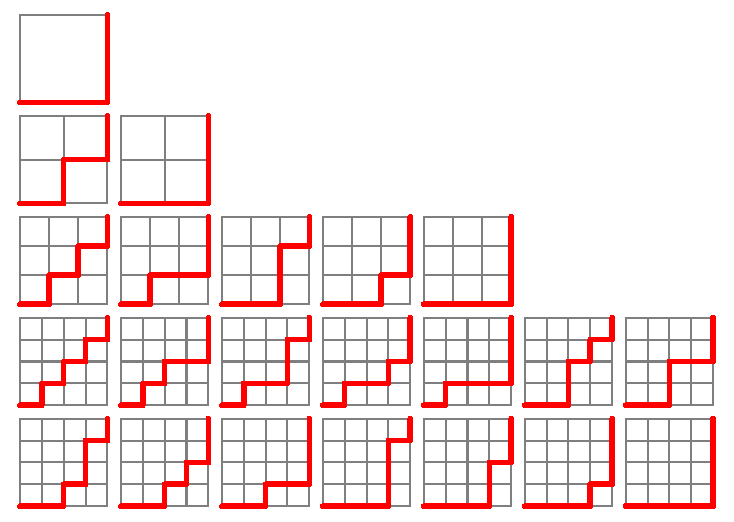
\includegraphics[width = 0.4\linewidth]{Dyck Path.pdf}
	\caption{Example walks for case $n=1\ (\#1),\ n=2\ (\#2),\ n=3\ (\#5), \ n=4\ (\#14)$ (\href{https://mathworld.wolfram.com/DyckPath.html}{Image Source})}
	\label{fig:dyckpath}
\end{figure}
\vspace{-1em}
\textbf{Problem Statement:}\\
Find the number of possible \emph{Dyck Path} for a given $n$ (for all test cases).
\begin{testcasesFunction}
	{$t$ \hfill(number of test cases, an integer)\\
	$n_1\ n_2\ \ldots n_t$ \hfill($t$ space seperated integers for each testcase)}
	{Number of Dyck Paths for $n_i$  \hfill(each test case on a newline)}
	{$1 \leq n_i \leq 15$}
	{\texttt{int dyck\_paths(int n)} -- returns the number of possible staircase walks for $n$.}
	{15\\1 2 3 4 5 6 7 8 9 10 11 12 13 14 15}
	{1\\2\\5\\14\\42\\132\\429\\1430\\4862\\16796\\58786\\208012\\742900\\2674440\\9694845}
	{https://github.com/paramrathour/CS-101/tree/main/Starter Codes/Dyck Path.cpp}
\end{testcasesFunction}